\documentclass[12pt]{article}

\usepackage[margin=12mm,left=7.5mm,right=7.5mm]{geometry}
\usepackage{hyperref,url,multicol,soul,hang,biblatex,changepage,multirow,longtable,xtab,array,textcomp,lipsum}
\usepackage[inline]{enumitem}
\usepackage{stoversymb}
%\usepackage{hanging}

\newcolumntype{C}{>{\centering\arraybackslash}m{27.5mm}}
\newcolumntype{D}{>{\centering\arraybackslash}m{23.75mm}}
\newcolumntype{G}{>{\raggedright\arraybackslash}m{22.5mm}}

\newcolumntype{H}{>{\centering\arraybackslash}m{23.5mm}}
\newcolumntype{J}{>{\centering\arraybackslash}m{17.5mm}}
%\newcolumntype{K}{>{\raggedright\arraybackslash}m{15.5mm}}

\newlength{\Oldarrayrulewidth}
\newcommand{\Cline}[2]{%
	\noalign{\global\setlength{\Oldarrayrulewidth}{\arrayrulewidth}}%
	\noalign{\global\setlength{\arrayrulewidth}{#1}}\cline{#2}%
	\noalign{\global\setlength{\arrayrulewidth}{\Oldarrayrulewidth}}}

\usepackage{xcolor}
\hypersetup{
	colorlinks=true,
	linkcolor={green!50!black},
	anchorcolor={green!60!black},
	urlcolor={red!90!black}%{blue!90!black}
	%citecolor={blue!50!black},
	%linkcolor,% [red]
	%anchorcolor,% [black]
	%citecolor,% [green]
	%filecolor,% [cyan]
	%menucolor,% [red]
	%runcolor,% [cyan - same as file color]
	%urlcolor={green!60!black}% [magenta]
}

\pagenumbering{gobble}

\setlength{\parskip}{1.25mm}

\newcommand{\iindent}{\hspace{6mm}}
\newcommand{\bb}[1]{\textbf{#1}}
\newcommand{\uln}[1]{{\noindent\ul{#1}}}
\newcommand{\vsp}{\vspace{0.75mm}}
\newcommand{\vspp}{\vspace{1.5mm}}
\newcommand{\vsppp}{\vspace{2.25mm}}
\newcommand{\vspppp}{\vspace{3mm}}
\newcommand{\rednote}[1]{{\footnotesize{\red{(#1)}}}}

\setlist[1]{topsep=0mm,itemsep=3mm,leftmargin=7.5mm,listparindent=6mm}
\setlist[2]{label=$\circ$,topsep=0mm,itemsep=1.5mm,leftmargin=7.5mm,listparindent=6mm,}
\setlist[3]{label=$-$,topsep=0mm,leftmargin=7.5mm,listparindent=6mm}


\begin{document}
	\part*{Data Structures}
	\section*{Complexity Summary}
	
	Discussion about complexity measures (big-$\Omega$, big-$\theta$, big-$O$) can be found at \href{https://www.programiz.com/dsa/asymptotic-notations}{Programiz}.
	
	Data in this table comes lots of places including:  \href{https://www.bigocheatsheet.com/}{Big-O Cheat Sheet},\ldots.\vspace{-4.5mm}
	
	\begin{center}
		\resizebox{\columnwidth}{!}{%
		\renewcommand{\arraystretch}{1.5}
		\begin{xtabular}{
		!{\vrule width 2pt}H
		!{\vrule width 2pt}J
		|J
		|J
		|J
		!{\vrule width 2pt}J
		|J
		|J
		|J
		!{\vrule width 2pt}J
		|J
		|J
		|J
		!{\vrule width 2pt}J
		!{\vrule width 2pt}}
			\noalign{\hrule height 2pt}
			\multirow{3}{*}{\textbf{Structure}} & 
			\multicolumn{4}{c!{\vrule width 2pt}}{\textbf{Best Case}} &
			\multicolumn{4}{c!{\vrule width 2pt}}{\textbf{Average Case}} &
			\multicolumn{4}{c!{\vrule width 2pt}}{\textbf{Worst Case}} &
			\multicolumn{1}{J!{\vrule width 2pt}}{\textbf{Space}} \\
			\cline{2-14}
			& 
			\multicolumn{1}{J|}{\textbf{\footnotesize{Access}}} &
			\multicolumn{1}{J|}{\textbf{\footnotesize{Search}}} & \multicolumn{1}{J|}{\textbf{\footnotesize{Ins}}} & 
			\multicolumn{1}{J!{\vrule width 2pt}}{\textbf{\footnotesize{Del}}} &
			\multicolumn{1}{J|}{\textbf{\footnotesize{Access}}} &
			\multicolumn{1}{J|}{\textbf{\footnotesize{Search}}} & \multicolumn{1}{J|}{\textbf{\footnotesize{Ins}}} & 
			\multicolumn{1}{J!{\vrule width 2pt}}{\textbf{\footnotesize{Del}}} &
			\multicolumn{1}{J|}{\textbf{\footnotesize{Access}}} &
			\multicolumn{1}{J|}{\textbf{\footnotesize{Search}}} & \multicolumn{1}{J|}{\textbf{\footnotesize{Ins}}} & 
			\multicolumn{1}{J!{\vrule width 2pt}}{\textbf{\footnotesize{Del}}} &
			\multicolumn{1}{J!{\vrule width 2pt}}{\textbf{\footnotesize{Worst}}} \\
			\noalign{\hrule height 2pt}
			\vspace{1.5mm}\hyperref[sec:Arrays]{{\footnotesize{Array}}} & $-$ & $-$ & $-$ & $-$ & $\theta(1)^1$ & $\theta(n)^1$ & $\theta(n)^1$ & $\theta(n)^1$ & $O(1)^1$ & $O(n)^1$ & $O(n)^1$ & $O(n)^1$ & $O(n)^1$\\
			\hline
			\vspace{1.5mm}\hyperref[sec:LinkedList]{{\footnotesize{Linked List}}} & $-$ & $-$ & $-$ & $-$ & $-$ & $-$ & $-$ & $-$ & $O(n)^1$ & $O(n)^{12}$ & $O(n)^{1}$ & $O(n)^1$ & $O(n)^1$\\
			\hline
			\vspace{2.5mm}\hyperref[sec:HashTable]{{\footnotesize{Hash Table}}\linebreak \scriptsize{Dictionary}} & $-$ & $-$ & $-$ & $-$ & $\theta(1)^1$ & $\theta(1)^1$ & $\theta(1)^1$ & $\theta(1)^1$ & $O(n)^1$ & $O(n)^1$ & $O(n)^1$ & $O(n)^1$ & $O(1)$ \\
			\hline
			\vspace{1.25mm}\hyperref[sec:BST]{{\footnotesize{BST}}} & $-$ & $O(1)^3$ & $O(1)^3$ & $O(n)^3$ & $-$ & $O(\log n)^{23}$ & $O(\log n)^{\star3}$ & $O(\log n)^3$ & $-$ & $O(n)^3$ & $O(n)^3$ & $O(n)^3$ & $O(n)^3$\\
			\hline
			\vspace{1.25mm}\hyperref[sec:AVL]{{\footnotesize{AVL tree}}} & $-$ & $-$ & $-$ & $-$ & $-$ & $O(\log n)^{4}$ & $O(\log n)^{4}$ & $O(\log n)^{4}$ & $-$ & $O(\log n)^{4}$ & $O(\log n)^{4}$ & $O(\log n)^{4}$ & $-$\\
			\hline
			\vspace{1.25mm}\hyperref[sec:RBT]{{\footnotesize{Red-Black tree}}} & $-$ & $-$ & $-$ & $-$ & $-$ & $-$ & $-$ & $-$ & $-$ & $-$ & $-$ & $-$ & $-$\\
			\hline
			\vspace{1.25mm}\hyperref[sec:Stack]{{\footnotesize{Stack}}} & $-$ & $-$ & $-$ & $-$ & $\theta(n)^{1}$ & $\theta(n)^{1}$ & $\theta(1)^{1}$ & $\theta(1)^{1}$ & $O(n)^{1}$ & $O(n)^{1}$ & $O(1)^{1}$ & $O(1)^{1}$ & $O(n)^{1}$\\
			\hline
			\vspace{1.25mm}\hyperref[sec:Queue]{{\footnotesize{Queue}}} & $-$ & $-$ & $-$ & $-$ & $\theta(n)^{1}$ & $\theta(n)^{1}$ & $\theta(1)^{1}$ & $\theta(1)^{1}$ & $O(n)^{1}$ & $O(n)^{1}$ & $O(1)^{1}$ & $O(1)^{1}$ & $O(n)^{1}$\\
			\noalign{\hrule height 2pt}
		\end{xtabular}}
	\end{center}
	\vspace{-9mm}
	\begin{flushleft}
		{\scriptsize{
			$^1$\href{https://www.bigocheatsheet.com/}{Big-O Cheat Sheet}\hspace{3mm}
			$^2$\href{https://techdevguide.withgoogle.com/paths/data-structures-and-algorithms/}{Google}\hspace{3mm}
			$^\star$Google says it's $O(n)$, but nothing else online agrees.\hspace{3mm}
			$^3$\href{https://iq.opengenus.org/time-and-space-complexity-of-binary-search-tree/}{OpenGenius IQ}\hspace{3mm}
			$^4$\href{https://en.wikipedia.org/wiki/AVL_tree}{AVL Wiki}
		}}
	\end{flushleft}

	\section*{Arrays}
	\label{sec:Arrays}
	\begin{itemize}
		\item Arrays allow storing elements of a single data type contiguously in memory.
		\begin{itemize}
			\item Random access is a great feature.
			\item Downside is that you must declare array size at creation, and they cannot dynamically grow.
			\item \textbf{Complexity:}
			
			\vsp
			
			\uln{Search:} 
			
			When unsorted, linear can be done in $O(n)$ time, $O(1)$ space.
			
			When sorted, binary can be done in $O(\log(n))$ time, $O(\log(n))$ space due to recursive calls.\vsp
			
			\uln{Insert:} 
			
			When unsorted, insert at the end can be done in $O(1)$ time, $O(1)$ space.
			
			When sorted, may require $O(n)$ time (because all elements may have to be moved), $O(1)$ space.\vsp
			
			\uln{Delete:} 
			
			When unsorted, delete is done by first linear searching, which requires $O(n)$ time, $O(1)$ space.
			
			When sorted, may require $O(n)$ time (because all elements may have to be moved), $O(\log(n))$ space (as an internal stack will be used).
		\end{itemize}
	\end{itemize}

	\section*{(Singly-)Linked Lists}
	\label{sec:LinkedList}
	\begin{itemize}
	\item Each node stores the element we want to store + a pointer to the next item in the linked list.
	\begin{itemize}
		\item This means that linked lists may take up more memory than an Array, because we have to store both the data \textit{and} the pointer while an Array has only the data stored.
	\end{itemize}
	\item Linked lists \textit{can} grow, because they're not stored contiguously.
	\begin{itemize}
		\item Upshot is that the size \textit{isn't} fixed: Linked Lists can grow dynamically.
		\item Downside is that random access isn't possible.
	\end{itemize}
	\item \textbf{Complexity:}
	
	\vsp
	
	\uln{Search / Access:} Both $O(n)$ time, as entire list must be traversed to reach desired element.\vsp
	
	\uln{Insert:} 
	\begin{itemize}
		\item Inserting at head position is $O(1)$ time, $O(1)$ space.
		\item Inserting at given position is $O(n)$ time, $O(1)$ space.
		\item Inserting after a given node is $O(1)$ time, $O(1)$ space.
		\item Inserting at end is $O(n)$ time, $O(1)$ space, though this can be made $O(1)$ time by keeping an extra pointer to the last node.
	\end{itemize}
	
	\uln{Delete:} 
	\begin{itemize}
		\item Deleting from head position is $O(1)$ time, $O(1)$ space.
		\item Deleting from middle is $O(n)$ time (both iterative and recursive), $O(1)$ space (if iterative) or $O(n)$ space if recursive (due to recursive call stack).
		\item Deleting from end is $O(n)$ time, $O(1)$ space, though this can be made $O(1)$ time by keeping an extra pointer to the last node.
	\end{itemize}
		
	\end{itemize}

	\section*{Hash Tables}
	\label{sec:HashTable}
	{\color{red}{In Python, one example is a \texttt{Dictionary}. Note: Google says maps/dictionaries are \textit{unordered}, but as of Python version 3.7, \texttt{Dictionary} objects are ordered.}}
	\begin{itemize}[topsep=3mm]
		\item The key idea of a hash table is to use a hash function to map keys to buckets. 
		\item Hash table is an array coupled with a hash function that takes the data (``key'') as input and outputs a hash value.
		\item Hash tables are theoretically better than linked lists, because they offer dynamic sizing while also allowing theoretically-constant insertion, deletion, and lookup times.
		\item One downside is collisions, which occur when the hash function returns the same index for two different keys. See the subsection on hash functions for more details about this.
		\item \textbf{Complexity:}
		
		\ul{Search / Access:} Best and average case are $O(1)$, worst cases is $O(n)$.\vsp
		
		\ul{Insert:} Best and average case are $O(1)$, worst cases is $O(n)$.\vsp
		
		\ul{Delete:} Best and average case are $O(1)$, worst cases is $O(n)$.\vsp
		
		\item There are two different kinds of hash tables: \textbf{Hash Sets} and \textbf{Hash Maps}.
	\end{itemize}

	\subsection*{Hash Functions}
	\begin{itemize}[topsep=0mm,itemsep=0mm,listparindent=6mm]
		\item When implementing hash tables, the best strategy is to choose a hash function that decreases the probability of collisions occurring. 
		\item A perfect hash function would be a one-to-one mapping between the keys and buckets. This would result in no collisions.
		
		However, in most cases, a hash function is not perfect, and there must be a trade-off between the number of buckets and the capacity of the buckets.
		\item Designing a good hash function is an open problem. Here are some properties of good hash functions:
		\begin{itemize}[topsep=0mm]
			\item Should make use of all info given by a key.
			\item Uniformly distributes across table.
			\item Maps similar keys to very different hash values.
			\item Uses only very fast operations.
		\end{itemize}
		\item Every hash function must have a built-in collision-resolution algorithm. Such an algorithm should solve the following problems:
		\begin{itemize}[topsep=0mm]
			\item How to organize the values in the same bucket?
			\item What if too many values are assigned to the same bucket?
			\item How to search for a target value in a specific bucket?
		\end{itemize}
		These questions are related to the capacity of the bucket and the number of keys which might be mapped into the same bucket according to our hash function.
		
		\item Here are some popular collision-resolution algorithms:
		\begin{itemize}[topsep=0mm,itemsep=3mm]
			\item \bb{Linear probing:} 
			
			If a key hashes to same index as a previously-stored key, it is assigned the next available slot in the table.\vsp
			
			\uln{Drawbacks:} Clustering. 
			
			Once a collision occurs, you increase the chances another will occur in the same area.\vsp
			
			\uln{Complexity:} 
			
			Worst-case is $O(n)$ for insertion, deletion, and lookups, as it's increasingly likely that the last slot in the table is the next available slot.
			
			\item \bb{Separate chaining:}
			
			The hash table is an array of pointers to linked lists. When collision occurs, the key can be inserted in constant time at the head of the appropriate linked list.\vsp
			
			\uln{Drawbacks:} Resolving collisions still requires a form of linear search, which is suboptimal. \vsp
			
			\uln{Complexity:} 
			
			Worst-case lookup is $O(n/k)$, where $k$ is the size of the hash table. 
			
			Note that theoretically $O(n/k)=O(n)$, so this isn't \textit{theoretically} better than the worst-case lookup time for a linked list. Realistically, however, $O(n/k)$ can be much better.
		\end{itemize}
	\end{itemize}

	\subsection*{Hash Sets}
	\begin{itemize}
			\item The hash set is one of the implementations of a set data structure to store no repeated values.
	\end{itemize}

	\subsection*{Hash Maps}
		\begin{itemize}
		\item The hash map is one of the implementations of a map data structure to store (key, value) pairs.
	\end{itemize}

	\section*{Trees, Tries, and Hybrid Tries}
	Much of the info about tries and hybrid tries comes more or less verbatim from \href{https://drstearns.github.io/tutorials/trie/}{this Dr. Sterns webpage}. There's also \href{https://stackoverflow.com/questions/11015320/how-to-create-a-trie-in-python}{this Stack Overflow thread} with different implementation possibilities, as well as \href{https://leetcode.com/problems/replace-words/solution/}{this leetcode exercise} which can be solved using tries in $O(n)$ time, $O(n)$ space (compared to $O(n^2)$ time, $O(n)$ space for the naive approach).
	
	\subsection*{Trees}
	\begin{itemize}
		\item Trees are non-linear, hierarchical data structures used to show relations using a parent-child hierarchy.
		
		They are considered to be some of the most powerful and advanced data structures, and are often employed to simplify and fasten searching and sorting operations.
		\item Linear structures like lists couldn't illustrate the nesting complexity of e.g. a directory file structure, a family tree, the HTML Document Object Model (DOM), etc.
		\item Trees are commonly used to represent game states in e.g. tic tac toe.
		\item Terminology:
		\begin{itemize}
			\item Each element is called a \emph{node}.
			\item The top node is called the \emph{root}.
			\item Any subnode of a given node is called a \emph{child node}, and the given node, in turn, is the child's \emph{parent}.
			
			Every child has only a single parent but a parent can have multiple child.
			\item \emph{Sibling nodes} are nodes on the same hierarchical level.
			\item Nodes higher than a given node in the same lineage are \emph{ancestors}, and those below it are \emph{descendants}.
			\item Nodes with no children are called \emph{leaves}.
			\item The \emph{height} of a tree is the length of the longest path to a leaf.
			\item The \emph{depth} of a node is the length of the path to its root.
		\end{itemize}
		\item If a tree has $n$ nodes, then it has $n-1$ edges. In the event that there are \textit{more} than $n-1$ edges, the structure is a graph, not a tree.
		\item \textbf{Methods to traverse trees:}
		
		Many search, etc. algorithms need the ability to traverse all the nodes in a given tree. There are several different strategies for tree traversal including:\vsp
			
		\uln{Breadth-First Traversal} or or \ul{Breadth-First Search (BFS)}: 
		
		In this method, we look at nodes at each level before looking at children.
		
		This method traverses the tree level-by-level and depth-by-depth. If we have a tree that's $2\leftarrow 1\rightarrow 5$, $3\leftarrow 2\rightarrow 4$, and $6\leftarrow 5\rightarrow 4$, for example, then BFS returns $1-2-5-3-4-6-7$.
		
		\uln{Depth-First Traversal} or \ul{Depth-First Search (DFS)}:
		
		In this method, we look at all descendants of a node before moving to the next node. \rednote{three versions of DFS are discussed below!}
		
		This method explores a path all the way to a leaf before backtracking and exploring another path. If we have a tree that's $2\leftarrow 1\rightarrow 5$, $3\leftarrow 2\rightarrow 4$, and $6\leftarrow 5\rightarrow 7$, for example, then DFS returns $1-2-3-4-5-6-7$.
	\end{itemize}

	\subsection*{Types of Trees}
	
	\subsubsection*{Generalities}
	\begin{itemize}
		\item A \emph{binary tree} is a tree in which each node has no more than two child nodes. One or both children may be null.
		\item An \emph{$n$-ary tree} is a tree in which each node has no more than $n$ child nodes. Any or all children may be null.
		
		Clearly, a binary tree is a 2-ary tree.
	\end{itemize}
	
	\subsubsection*{Binary Search Trees (BSTs)}
	\label{sec:BST}
	
	A BST is a binary tree that satisfies a specific ordering property, namely that any/all left nodes (on any given subtree) are less than the root node, which are less than any/all right nodes.\vsp
	
	\uln{Searches/Finds:} \begin{itemize}\item[]This property of BST yields efficient searches/finds, because at each operation, we've chopped off $\approx$ half of the nodes.\end{itemize}
	
	\uln{Insertions:} Insertion works similar to searches/finds.
		
	\begin{itemize}\item[]One possible issue that could result from this is that the resulting tree can become super-unbalanced; think of inserting 1, then 2, then 3, etc., which essentially turns your BST into a linked list.\end{itemize}
	
	\uln{Traversing:} There are three main types of traversals. \rednote{all of these are examples of DFS!}\vspace{-1.5mm}
	
	{\scriptsize{(assume that $B$ is the root, $A$ is its left child, and $C$ is its right child)}}
	\begin{itemize}[leftmargin=15mm,label=$\circ$]
		\item \textit{pre-order} traversal, which means you visit the root first, then its left nodes, then its right nodes. In other words, $B\rightarrow A\rightarrow C$.
		\item \textit{in-order} traversal, which means you visit the left nodes first, then the current node, then the right nodes. In other words, $A\rightarrow B\rightarrow C$. \rednote{these are usually preferred with BSTs because the nodes are printed in order.}
		
		\textbf{Example use:} To determine if a tree is a valid BST, you can use in-order traversal to record the nodes in order and then see if left nodes are less than parents are less than right nodes, i.e. if \texttt{x[i]<x[i+1]} for all \texttt{i=0,1,\ldots,len-1}.
		\item \textit{post-order} traversal, which means you visit the left nodes first, then the right nodes, then the current node. In other words, $A\rightarrow C\rightarrow B$.
	\end{itemize}\vspp
		
	\noindent\textbf{Complexity:}
	
	According to \href{https://iq.opengenus.org/time-and-space-complexity-of-binary-search-tree/}{OpenGenius IQ} (and supported by other sources as well):
	\begin{center}
		\renewcommand{\arraystretch}{1.5}
		\begin{tabular}{|l|c|c|c|c|}
			\hline
			\textbf{Operation} & \textbf{Worst Case} & \textbf{Average Case} & \textbf{Best Case} & \textbf{Space} \\
			\hline
			Search & $O(n)$ & $O(\log n)$ & $O(1)$ & $O(n)$ \\
			\hline
			Insert & $O(n)$ & $O(\log n)$ & $O(1)$ & $O(n)$ \\
			\hline
			Delete & $O(n)$ & $O(\log n)$ & $O(n)$ & $O(n)$ \\
			\hline
		\end{tabular}
	\end{center}
	Along the same lines, multiple sources have claimed that:\vspp
	
	\ul{Search:} $O(\log n)$ if balanced, $O(n)$ if unbalanced. Average: $O(\log n)$. \rednote{Google agrees....}\vspp
		
	\ul{Insert:} $O(\log n)$ if balanced, $O(n)$ if unbalanced. Average: $O(\log n)$. \rednote{Google says $O(n)$ instead....}\vspp
	
	\noindent However, Google says that the average-time insertion into a BST is $O(n)$:
	
	\begin{center}
		\fbox{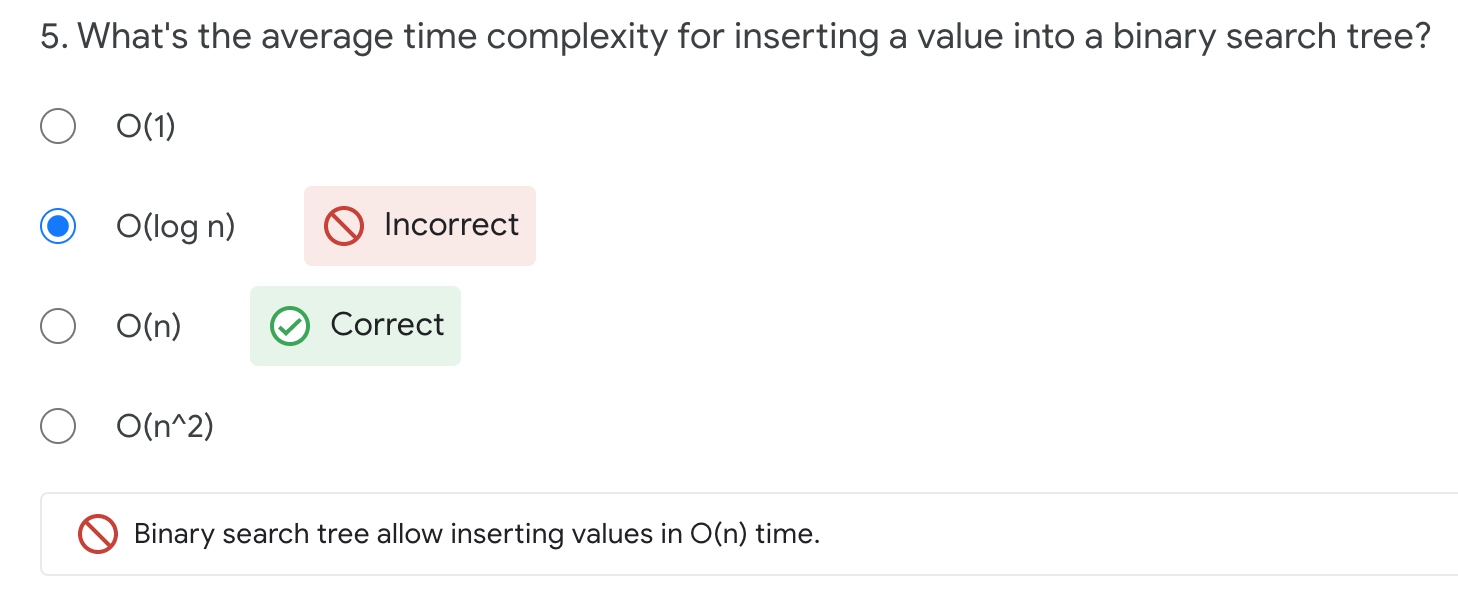
\includegraphics[scale=0.5]{img/google1.png}}
	\end{center}
	
	\subsubsection*{AVL (Adelson-Velshi and Landis) Trees}
	\label{sec:AVL}
	
	An AVL tree is a self-balancing BST.
	
	In an AVL tree, the heights of the two child subtrees of any node differ by at most one; if at any time they differ by more than one, re-balancing is done to restore this property.\vspp
	
	\noindent\textbf{Relation to \hyperref[sec:RB]{Red-Black (RB) Trees}:}
	
	Every AVL tree can be colored red-black, but there exist RB trees that \emph{are not} AVL-balanced.]\vspp
	
	\noindent\textbf{Complexity:}
	
	Lookup, insertion, and deletion all take $O(\log n)$ time in both the average and worst cases (where $n$ is the number of nodes in the tree prior to the operation). Insertions and deletions may require the tree to be re-balanced by one or more tree rotations.\vspp
	
	\noindent\textbf{Rebalancing:}
	
	During insert and delete operations, a (temporary) height difference of 2 may arise, which means that the parent subtree has to be ``rebalanced''. 
	
	The given repair tools are the so-called \emph{tree rotations}, because they move the keys only ``vertically,'' so that the (``horizonta'') in-order sequence of the keys is fully preserved (an essential necessity for a BST).

	Let $X$ be the node that has a (temporary) balance factor of $−2$ or $+2$. Its left or right subtree was modified. Let $Z$ be the higher child (see figures 2 and 3). Note that both children are in AVL shape by induction hypothesis.
	
	There are four possible variants of the violation, each with its own solution.
	\begin{enumerate}[label=(\roman*),leftmargin=16.5mm]
		\item \ul{Right Right}. $Z$ is a right child of its parent $X$ and $BF(Z)\geq 0$. In this case, $X$ is re-balanced with a \texttt{rotate\_Left} simple rotation. See AVL Figure 2.
	
		\item \ul{Left Left}. $Z$ is a left child of its parent $X$ and $BF(Z)\leq 0$. In this case, $X$ is re-balanced with a \texttt{rotate\_Right} simple rotation. See (the mirror image of) AVL Figure 2.
		
		\item \ul{Right Left}. $Z$ is a right child of its parent $X$ and $BF(Z)< 0$. In this case, $X$ is re-balanced with a \texttt{rotate\_RightLeft} double rotation. See AVL Figure 3.
		
		\item \ul{Left Right}. $Z$ is a left child of its parent $X$ and $BF(Z) > 0$. In this case, $X$ is re-balanced with a \texttt{rotate\_LeftRight} double rotation. See (the mirror image of) AVL Figure 3.
	\end{enumerate}
	
	\begin{minipage}[b]{0.5\textwidth}
		\centering
		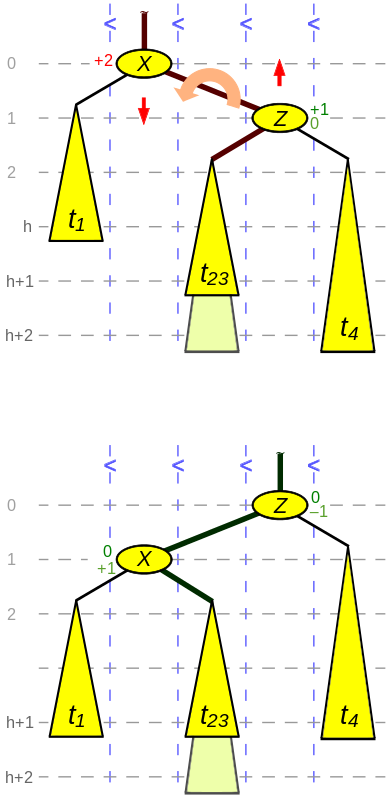
\includegraphics[height=125mm]{img/avl2.png}
		
		\textit{AVL Figure 2}
	\end{minipage}\hspace{3mm}
	\begin{minipage}[b]{0.5\textwidth}
		\centering
		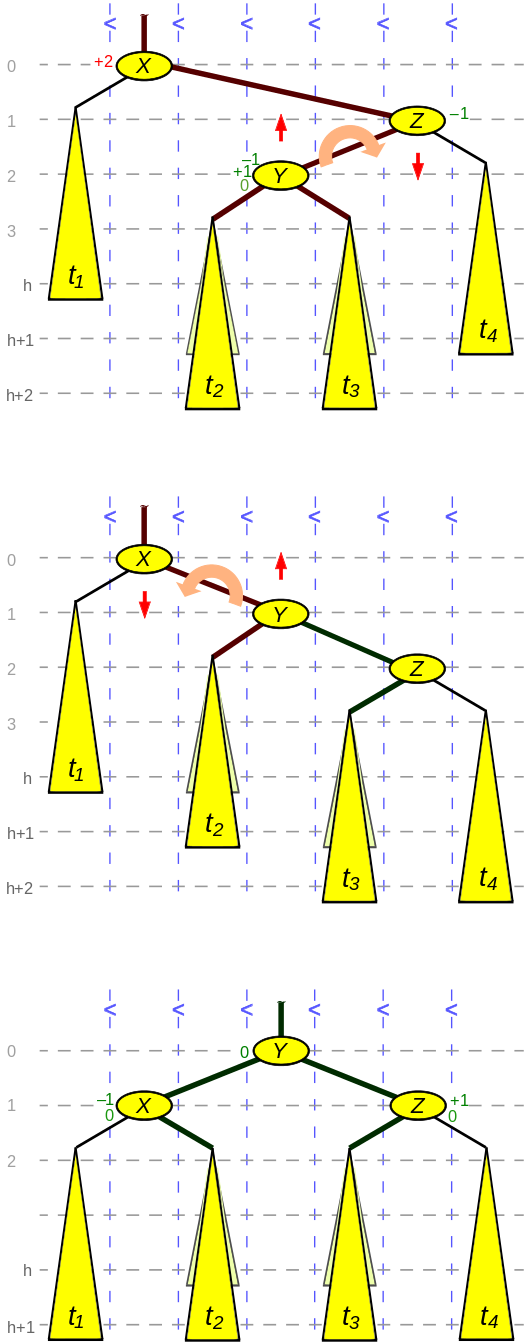
\includegraphics[height=175mm]{img/avl3.png}
		
		\textit{AVL Figure 3}
	\end{minipage}\hspace{3mm}

	\subsubsection*{Red-Black Trees}
	\label{sec:RB}
	
	\noindent\textbf{Relation to \hyperref[sec:AVL]{AVL Trees}:} 
	
	Every AVL tree can be colored red-black, but there exist RB trees that \emph{are not} AVL-balanced.\vspp
	
	\red{\lipsum[1]}
	
	\subsection*{Tries}
	
	In computer science, a \textbf{trie} (also known as a \emph{digital tree} or \emph{prefix tree}) is a tree data structure used for locating specific keys from within a set. It is an example of a $k$-ary search tree.
	
	Like other search-oriented data structures, a trie stores keys and associated values. Together, the key and value are called an entry. The keys are most often strings, with links between nodes defined by individual characters, but the value could be of any type, as the trie just stores and retrieves it as an opaque value. Often this value is a unique identifier or pointer that gets you to some data related to the key (e.g. the primary key of a record in a DBMS).
	
	In order to access a key, the trie is \ul{traversed depth-first}, following the links between nodes. The links represent characters in the key.
	
	This is very useful for things like dictionaries:
	
	\begin{center}
		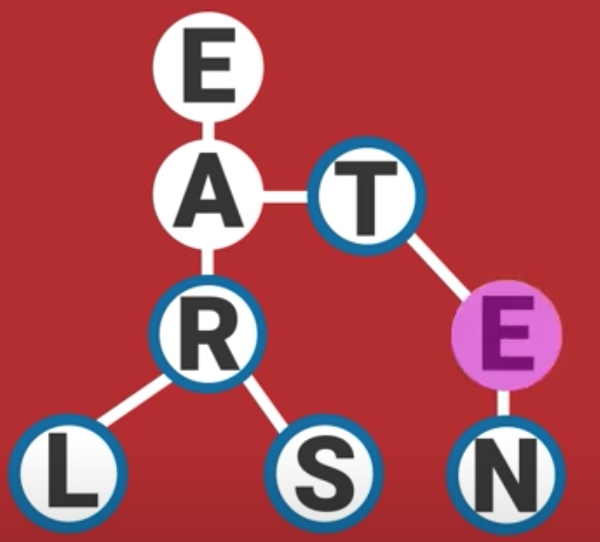
\includegraphics[scale=0.5]{img/trie.png}\vspace{1.5mm}
		
		\parbox{4in}{\centering\textit{For word \texttt{EAR},make \texttt{E}\textrightarrow \texttt{A}\textrightarrow \texttt{R}; from there, make \texttt{EARS}, \texttt{EARL}, etc., or branch off of \texttt{EA} to make \texttt{EAT}, \texttt{EATEN}, etc. The blue outlines note an identifier that indicates that the nodes are valid word-enders.}}
	\end{center}
		
	The height of a trie is always equal to the length of the longest key added to it. This means that tries tend to be very wide and not terribly deep, which makes retrieval speed much quicker. Adding a new key requires creating at most \texttt{len(key)} nodes, but if your keys share common prefixes (which is typical), you will re-use nodes from previously-added keys.
		
	\textbf{Similarities with maps.} Like a map, a trie can also be used to store only keys with no associated values. For example, a simple list of dictionary words might not need associated values, but you might want to find all words that start with a given prefix. In these cases we use a variant of a trie that only stores keys with no associated values. The structure is similar, but we can save a little memory in each node.
	
	\textbf{Contrasts with BSTs.} Unlike a binary search tree, nodes in the trie do not store their associated key. Instead, a node's position in the trie defines the key with which it is associated. This distributes the value of each key across the entire data structure, meaning that not every node necessarily has an associated value.
	
	\subsubsection*{Adding Keys and Values}
	A trie constructs a tree of nodes based on the letters in the keys added to it. The tree starts with a single root node that holds no values. When a new key/value pair is added, the trie follows this algorithm:
	\begin{enumerate}[itemsep=0mm]
		\item let current node = root node
		\item for each letter in the key,
		\begin{enumerate}
			\item find the child node of current node associated with that letter
			\item if there is no child node associated with that letter, create a new node and add it to current node as a child associated with the letter
			\item set current node = child node
		\end{enumerate}
		\item add value to current node
	\end{enumerate}
	
	When indexing keys that are not unique (e.g., last names), we will often need to add the same key to the trie multiple times but with different values. For example, this shows \emph{go} with value 1, \emph{git} with value 2, \emph{gob} with value 3, and (a repeat) \emph{go} with value 4:
	
	\begin{center}
		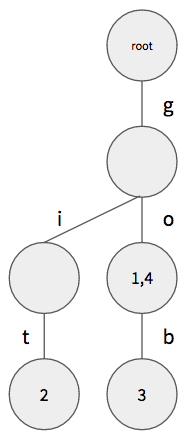
\includegraphics[scale=0.5]{img/trie4.png}
	\end{center}

	\subsubsection*{Retrieving Keys and Values}
	
	Tries generally allow very fast retrieval of keys starting with a prefix. To do so, follow this algorithm:
	\begin{enumerate}[itemsep=0mm]
		\item let current node = root node
		\item for each letter in the prefix,
		\begin{enumerate}
			\item find the child node of current node associated with that letter
			\item if there is no child associated with that letter, no keys start with the prefix, so return an empty/null list
			\item set current node = child node
		\end{enumerate}
		\item current node now points to the branch containing all keys that start with the prefix; recurse down the branch, gathering the keys and values, and return them
	\end{enumerate}

	Finding the start of the branch containing all keys and values takes at most \texttt{len(prefix)} lookups, regardless of how many entries there are in the trie. 
	
	Retrieval complexity depends on the length of the key prefix, not the number of entries in the trie, so the retrieval performance remains about the same as we add more entries. Compare that with a binary search tree, which requires at most $log(n)$ comparisons to find the first matching key (where $n$ is the number of entries in the tree).
	
	Branches for a short prefix might contain a lot of keys and values, so we typically return only the first $m$ entries from the branch (where $m$ is a usually-small parameter passed by the caller. To get this subset, you do a \ul{depth-first recursion} down the branch, following the letters in each node according to their alphabetical order. As soon as you gather $m$ keys and values, you return to stop the recursion.
	
	\subsection*{Hybrid Tries}
	
	Tries offer fast retrieval, but they aren't very space-efficient unless most keys are short and share common prefixes (i.e., dictionary words). Longer keys that don't share many prefixes create a ``leggy'' tree structure which resembles a many-tentacled octopus!
	
	In these situations, it's common to use a variant known as a hybrid trie. Instead of always creating a new node for each letter in the key, the leaf nodes in a hybrid trie store a list of key suffixes until those reach some maximum number, for example, 50. When the 51st key is added, the leaf node then transforms itself into a typical trie node, and creates a new leaf node for each distinct first-letter in the key suffixes it holds. Each of the new child leaf nodes then stores what remains of the key suffixes for their respective letter.
	
	For example, consider the following:
	
	\begin{center}
		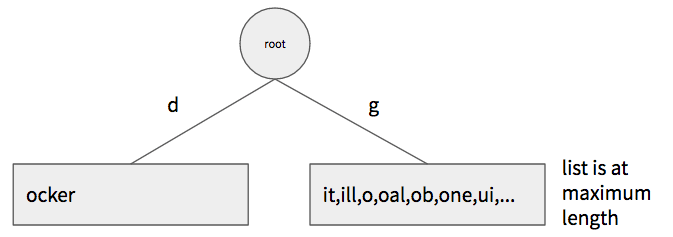
\includegraphics[scale=0.5]{img/hybrid-trie-1.png}
	\end{center}
	From here, adding \emph{guard} won't work because the right child is full, so...
	\begin{center}
		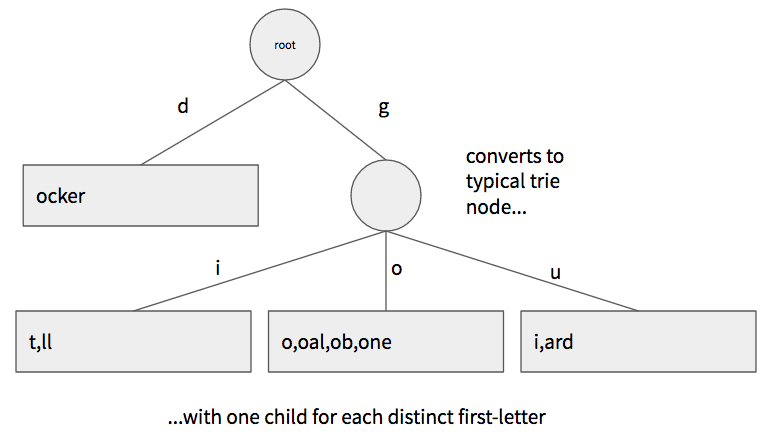
\includegraphics[scale=0.5]{img/hybrid-trie-2.png}
	\end{center}
	...adding \emph{guard} turns the first level into a traditional trie structure and moves the hybrid part one level down.
	
	\textbf{Note:} These diagrams depict only the keys, but you can create a hybrid trie that also stores associated values. The leaf nodes would store key-suffix and value pairs instead of just the key suffixes.
	
	\section*{Stacks and Queues}
	\subsection*{Stacks and DFS}
	\label{sec:Stack}
	\begin{itemize}
		\item Stacks are like stacks of plates: Last in, first out (LIFO).
		
		\begin{itemize}
			\item The insert operation for a stack is called \emph{push}. Inserting always happens at the end.
			\item The delete for a stack is called \emph{pop}. Removing always happens from the end.
		\end{itemize}
		\begin{center}
			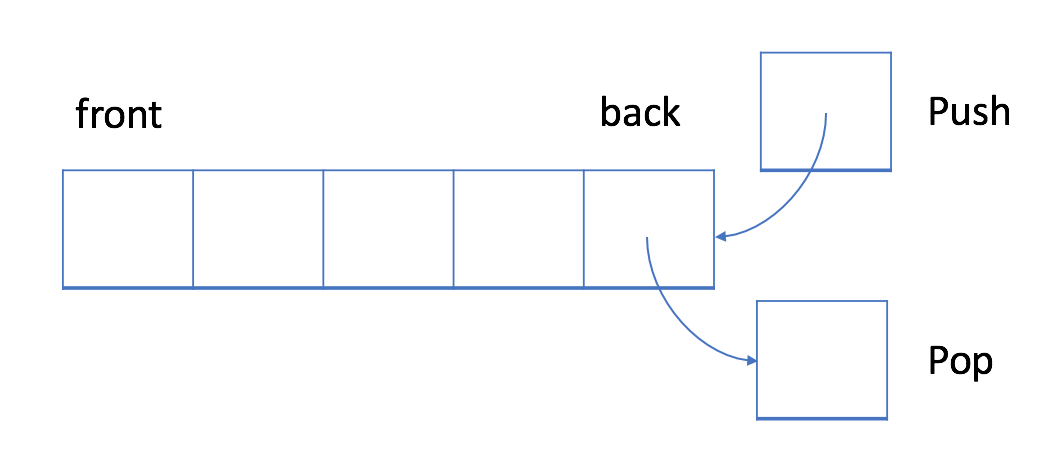
\includegraphics[scale=0.5]{img/PushPop.png}
		\end{center}
	
		\item Stacks are even easier to implement than queues using any sort of dynamic array.
		
		\item A so-called \texttt{minstack} can be implemented which supports \emph{push}, \emph{pop}, \emph{peek} (at the top element), and \emph{getMin()}. 
		
		This can be done \href{https://leetcode.com/problems/min-stack/discuss/2281964/Java-Solution}{with two stacks simultaneously} by pushing on to \texttt{stack2} the smallest elements pushed on to \texttt{stack1} and by popping from \texttt{stack2} any elements equal to pops done on \texttt{stack1}.
		
		This may also be doable using \href{https://leetcode.com/problems/min-stack/discuss/2281796/C%2B%2B-One-stack-Solution}{only one stack} if we push/pop pairs of elements, one of which is a tracker for the existing min.
		
		Does this mean \texttt{maxstack}, \texttt{avg stack}, etc., can also be done? 
		
		\item Stacks are commonly used when doing a depth-first search (DFS).\footnote{This process works for general graphs as well as trees, as described in subsequent passages.}
		\begin{itemize}
			\item In the first round, the root node is processed. In the second round, choose a path a neighboring node and trace-back until a node is reached with no way to go deeper. Then, backtrack to the root and choose a new path to a new second node. From there, try subsequent paths until hitting a node that's already been visited; then, backtrack and start again.
			
			The processing order of the nodes is the exact opposite order as how they were added to the stack, which is Last-in-First-out (LIFO). That's why we use a stack in DFS.
			
			\item Different from BFS, the nodes visited earlier might not be the nodes which are closer to the root node. As a result, the first path found in DFS might not be the shortest path.
		\end{itemize}
		\item While it may seem like stacks are unnecessary when implementing DFS recursively, even recursive implementations use an implicit stack provided by the system. This is known as \textbf{the Call Stack}.
		
		\item The advantage of the recursion solution is that it is easier to implement. However, there is a huge disadvantage: if the depth of recursion is too high, a stack overflow will result. In that case, BFS may be a good solution, as may implementing DFS using an explicit stack.
		
		\item Stacks can be used to implement queues (next section), but doing so requires $\geq 2$ stacks.
	\end{itemize}

	\subsection*{Queues and BFS}
	\label{sec:Queue}
	\begin{itemize}
		\item Queues are like lines at the movies: First in, first out (FIFO).
		
		\begin{itemize}
			\item The insert operation for a queue is called \emph{enqueue}. Inserting always happens at the end.
			\item The delete for a queue is called \emph{dequeue}. Removing always happens from the front.
		\end{itemize}
		\begin{center}
			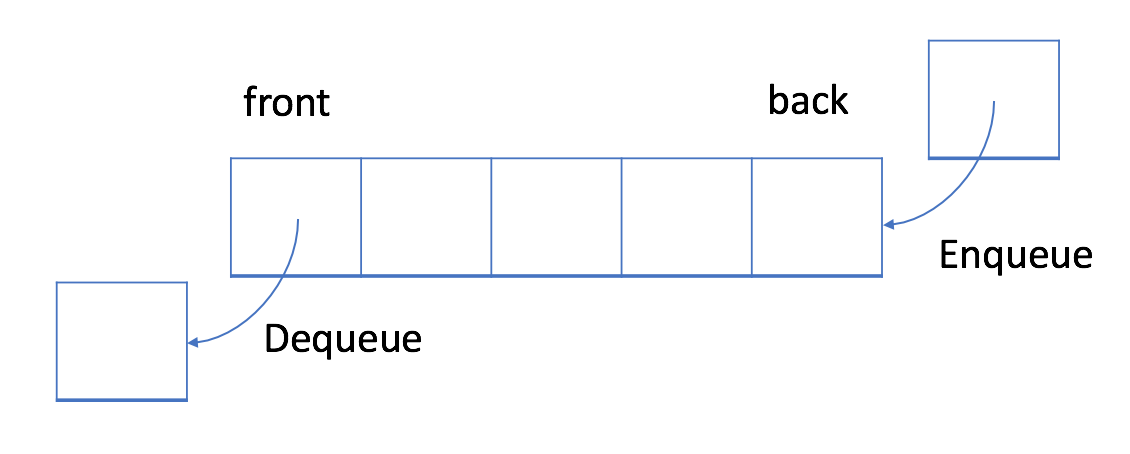
\includegraphics[scale=0.5]{img/EnDeQueue.png}
		\end{center}
	
		\item Queues are easy to implement using e.g. \texttt{ArrayList}s in Java. However, the naive implementation may be inefficient in some cases, as the movement of the start pointer means more and more space will be wasted. This will be unacceptable when facing a space limitation.
		
		\item Even better than this linear implementation is a \emph{circular} implementation: This can be done using a circularly-linked list, i.e. an array and two pointers, \texttt{head} (indicating the starting position) and \texttt{tail} (indicating the ending position).
		
		\item Queues are commonly used when doing a breadth-first search (BFS).\footnote{This process works for general graphs as well as trees, as described in subsequent passages.}
		
		\begin{itemize}
			\item In the first round, we process the root node. In the second round, we process the nodes next to the root node. In the third round, we process the nodes which are two steps from the root node; so on and so forth.
			
			Similar to tree's level-order traversal, the nodes closer to the root node will be traversed earlier.
			
			\item If a node $X$ is added to the queue in the $k$th round, the length of the shortest path between the root node and $X$ is exactly $k$. 
			
			That is to say, you are already in the shortest path the first time you find the target node.
			
			\item The root node is enqueued first. Then in each round, we process the nodes which are already in the queue one-by-one and add all their neighbors to the queue. \textbf{Note:} The newly-added nodes will \emph{not} be traversed immediately but will be processed in the next round.
			
			The processing order of the nodes is the exact same order as how they were added to the queue, which is FIFO. That's why queues are used for breadth-first searches!
			
			\item Sometimes, the naive implementation will be problematic, and you'll have to ensure you never visit the same node twice (lest we get stuck in an infinite loop, like if our graph has a cycle).
			
			To avoid this, you can combine a hash table (hash set in particular) to the fray, \href{https://leetcode.com/explore/learn/card/queue-stack/231/practical-application-queue/1372/}{as shown here}. Sometimes, this is unnecessary: In tree traversal, for example, or if you want to add a node to the queue multiple times.
		\end{itemize}
	\end{itemize}

	\subsubsection*{Priority Queues}
	
	\begin{itemize}
		\item A priority queue is a special type of queue in which each element is associated with a priority value. 
		
		\item In a (normal) queue, the first-in-first-out rule is implemented; in a priority queue, the values are removed on the basis of priority. 
		
		\emph{Priorities queues can be implemented to first remove values with the highest or lowest associated priority}.\footnote{If elements with the same priority occur, they are served according to their order in the queue.}
		
		\item Priority queue can be implemented using an array, a linked list, a heap, or a binary search tree. Among these data structures, heaps provide an efficient implementation of priority queues.
		
		Here are complexity comparisons of the various data structures, according to \href{https://www.programiz.com/dsa/priority-queue}{Programiz} and (for building) \href{https://en.wikipedia.org/wiki/Priority_queue}{Wikipedia}:
		
		\begin{center}
			\renewcommand{\arraystretch}{1.5}
			\begin{tabular}{|l|>{\centering\arraybackslash}m{22mm}|>{\centering\arraybackslash}m{22mm}|>{\centering\arraybackslash}m{22mm}|>{\centering\arraybackslash}m{22mm}|}
				\hline
				\textbf{Operation} & \textbf{Peek} & \textbf{Enqueue} & \textbf{Dequeue} & \textbf{Building} \\
				\hline
				Linked List & $O(1)$ & $O(n)$ & $O(1)$ & $-$\\
				\hline
				Binary Heap & $O(1)$ & $O(\log n)$ & $O(\log n)$ & $O(n)$ \\
				\hline
				Binary Search Tree & $O(1)$ & $O(\log n)$ & $O(\log n)$ & $O(n\log n)$\\
				\hline
			\end{tabular}
		\end{center}
	
		\item As discussed on \href{https://en.wikipedia.org/wiki/Priority_queue}{Wikipedia}, priority queues can be used to sort and can be implemented using around a dozen different data structures (including some very specialized heaps such as \href{https://en.wikipedia.org/wiki/Van_Emde_Boas_tree}{\emph{van Emde Boas trees}} and \href{https://en.wikipedia.org/wiki/Fusion_tree}{\emph{fusion trees}}).
		
		There is also \href{https://en.wikipedia.org/wiki/Priority_queue#Summary_of_running_times}{an entire section} on the time complexities of various heap data structures (which are not copied here because of how specialized they are).
	\end{itemize}
	
	\part*{Search Algorithms}
	
	\section*{Basics \& Terminology}
	
	\begin{itemize}
		\item A search algorithm is said to be \emph{in-place} if it does not need an extra space, i.e. if it produces an output in the same memory that contains the data being sorted.
		
		This is done by transforming the input ``in-place,'' so extra memory is not needed (though a small constant amount of extra space used for variables is allowed).
		
		\item A sorting algorithm is said to be \emph{stable} if two objects with equal keys appear in the same order after sorting as they appear in the input array pre-sorting.
	\end{itemize}
	
	\section*{Complexity Summary}
	
	Most of the table summaries come from \href{https://www.geeksforgeeks.org/time-complexities-of-all-sorting-algorithms/}{GeeksForGeeks}.
	
	\begin{center}
	\renewcommand{\arraystretch}{2.5}
	\begin{xtabular}{!{\vrule width 2pt}C!{\vrule width 2pt}D|D|D!{\vrule width 2pt}D!{\vrule width 2pt}G!{\vrule width 2pt}}
		\noalign{\hrule height 2pt}
		\multirow{3}{*}{\textbf{Algorithm}} & 
		\multicolumn{3}{c!{\vrule width 2pt}}{\textbf{Time Complexity}} &
		\multicolumn{1}{c!{\vrule width 2pt}}{\parbox{25mm}{\centering\textbf{\vphantom{o}\\Space\\Complexity\\\vphantom{o}}}} & 
		\multicolumn{1}{c!{\vrule width 2pt}}{\multirow{3}{*}{\textbf{Notes}\vspace{6mm}}} \\
		\cline{2-5}
		& 
		\multicolumn{1}{D|}{\textbf{Best}} & \multicolumn{1}{D|}{\textbf{Average}} & 
		\multicolumn{1}{D!{\vrule width 2pt}}{\textbf{Worst}} &
		\multicolumn{1}{D!{\vrule width 2pt}}{\textbf{Worst}} & \\
		\noalign{\hrule height 2pt}
		\hyperref[sec:SelSort]{\vspace{1mm}\newline Selection Sort} & $\Omega(n^2)$ & $\theta(n^2)$ & $O(n^2)$ & $O(1)$ & {\footnotesize{\vspace{2mm}not stable, in-place}} \\
		\hline
		\hyperref[par:StSelSort]{\vspace{1mm}\newline Stable Selection Sort} & $\Omega(n^2)$ & $\theta(n^2)$  & $O(n^2)$ & $O(1)$ & {\footnotesize{\vspace{3mm}stable, in-place}} \\
		\hline
		\hyperref[sec:BubSort]{Bubble Sort} & $\Omega(n)$ & $\theta(n^2)$ & $O(n^2)$ & $O(1)$ & \\
		\hline
		\hyperref[sec:InsSort]{Insertion Sort} & $\Omega(n)$ & $\theta(n^2)$ & $O(n^2)$ & $O(1)$ & \\
		\hline
		\hyperref[sec:HeapSort]{Heap Sort} & $\Omega(n\log n)$ & $\theta(n\log n)$ & $O(n\log n)$ & $O(1)$ & \\
		\hline
		\hyperref[sec:QSort]{Quick Sort} & $\Omega(n\log n)$ & $\theta(n\log n)$ & $O(n^2)$ & $O(\log n)$ & \\
		\hline
		\hyperref[sec:MerSort]{Merge Sort} & $\Omega(n\log n)$ & $\theta(n\log n)$ & $O(n\log n)$ & $O(n)$ & \\
		\hline
		\hyperref[sec:BuckSort]{Bucket Sort} & $\Omega(n+k)$ & $\theta(n+k)$ & $O(n^2)$ & $O(n)$ & \\
		\hline
		\hyperref[sec:RadSort]{Radix Sort} & $\Omega(nk)$ & $\theta(nk)$ & $O(n+k)$ & $O(nk)$ & \\
		\hline
		\hyperref[sec:CntSort]{Count Sort} & $\Omega(n+k)$ & $\theta(n+k)$ & $O(n+k)$ & $O(k)$ & \\
		\hline
		\hyperref[sec:ShSort]{Shell Sort} & $\Omega(n)$ & $\theta(n\log n)$ & $O(n\log n)$ & $O(1)$ & \\
		\hline
		\hyperref[sec:TimSort]{Tim Sort} & $\Omega(n)$ & $\theta(n^2\log^2(n))$ & $O(n^2\log^2(n))$ & $O(n)$ & \\
		\hline
		\hyperref[sec:TrSort]{Tree Sort} & $\Omega(n\log n)$ & $\theta(n\log n)$ & $O(n^2)$ & $O(n)$ & \\
		\hline
		\hyperref[sec:CubeSort]{Cube Sort} & $\Omega(n)$ & $\theta(n\log n)$ & $O(n\log n)$ & $O(n)$ & \\
		\noalign{\hrule height 2pt}
	\end{xtabular}
	\end{center}
	
	\section*{Individual Algorithms}
	
	Here, we collect details for all (well, \textit{most}...) of the sorting algorithms commonly encountered.
	
	\subsection*{Selection Sort}
	\label{sec:SelSort}
	
	Extended analysis done \href{https://www.geeksforgeeks.org/selection-sort/}{here}.
	
	The selection sort algorithm sorts an array by repeatedly finding the minimum element from the currently-unsorted part and putting it at the beginning. 
	
	The algorithm maintains two subarrays in a given array: \begin{enumerate*}[label=(\roman*)]\item a subarray which is already sorted, and \item the remaining subarray which is unsorted\end{enumerate*}. In every iteration of selection sort, the minimum element from the unsorted subarray is picked and moved to the sorted subarray.
	
	\textbf{Example:} Start with the array \texttt{\{64,25,12,22,11\}}: \vspace{-2.25mm}
	\begin{verbatim}
	      Step 1: Traverse whole list to find minimium = 11.
	      Step 2: Swap element 1 for 11. Result: {11,25,12,22,64}.
	      Step 3: Traverse list starting at 25 to find minimum = 12.
	      Step 4: Swap element 2 for 12. Result: {11,12,25,22,64}.
	      Step 5: Traverse list starting at 25 to find minimum = 22.
	      Step 6: Swap element 3 for 22. Result: {11,12,22,25,64}.
	      Step 7: Traverse list starting at 25 to find minimum = 25. Do nothing.
	      Step 8: Traverse list starting at 64 to find minimum = 64. Do nothing.
	\end{verbatim}

	\begin{itemize}[]
		\item \textbf{Complexity:} The complexity here is $O(n^2)$, since you need one loop to select an element of the array followed by a second to compare that element with all the others.
	
		\item \textbf{Stability:} This algorithm \textit{isn't} stable. 
	
		However, it can be made stable by implementing \label{par:StSelSort}\href{https://www.geeksforgeeks.org/stable-selection-sort/}{stable seleection sort} instead. The idea here is: Instead of swapping, the minimum element may be placed in its final position by placing the number in the desired position and then pushing every subsequent element one step forward (instead of swapping).
	
		This is similar to the methodology employed by \hyperref[sec:InsSort]{Insertion Sort}.
	\end{itemize}
	
	\subsection*{Bubble Sort}
	\label{sec:BubSort}
	
	\red{\lipsum[1]}
	
	\subsection*{Insertion Sort}
	\label{sec:InsSort}
	
	\red{\lipsum[1]}
		
	\subsection*{Heap Sort}
	\label{sec:HeapSort}
	
	\red{\lipsum[1]}
	
	\subsection*{Quick Sort}
	\label{sec:QSort}
	
	\red{\lipsum[1]}
	
	\subsection*{Merge Sort}
	\label{sec:MerSort}
	
	\red{\lipsum[1]}
	
	\subsection*{Bucket Sort}
	\label{sec:BuckSort}
	
	\red{\lipsum[1]}
	
	\subsection*{Radix Sort}
	\label{sec:RadSort}
	
	\red{\lipsum[1]}
	
	\subsection*{Count Sort}
	\label{sec:CntSort}
	
	\red{\lipsum[1]}
	
	\subsection*{Shell Sort}
	\label{sec:ShSort}
	
	\red{\lipsum[1]}
	
	\subsection*{Tim Sort}
	\label{sec:TimSort}
	
	\red{\lipsum[1]}
	
	\subsection*{Tree Sort}
	\label{sec:TrSort}
	
	\red{\lipsum[1]}
	
	\subsection*{Cube Sort}
	\label{sec:CubeSort}
	
	\red{\lipsum[1]}
\end{document}